\begin{figure}
    \centering
    \subfloat[Number of GSS edges.]{
        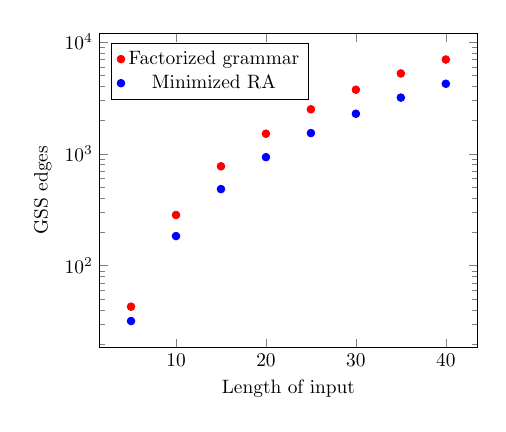
\begin{tikzpicture}[scale=0.7]
        \begin{axis}[
        legend pos = north west,
        xlabel = {Length of input},
        ylabel = {GSS edges},
        ymode=log
        ]
        \addplot [only marks, red] coordinates {
            (5,43) (10,284) (15,774) (20,1514) (25,2504) (30,3744) (35,5234) (40,6974)
        };
        \addplot [only marks, blue] coordinates {
            (5,32) (10,184) (15,484) (20,934) (25,1534) (30,2284) (35,3184) (40,4234)
        };
        \legend{ 
            Factorized grammar, 
            Minimized RA
        };
        \end{axis}
        \end{tikzpicture}
        \label{fig:GSSedges}
    }
    ~
    \subfloat[Time of parsing without SPPF construction.]{
        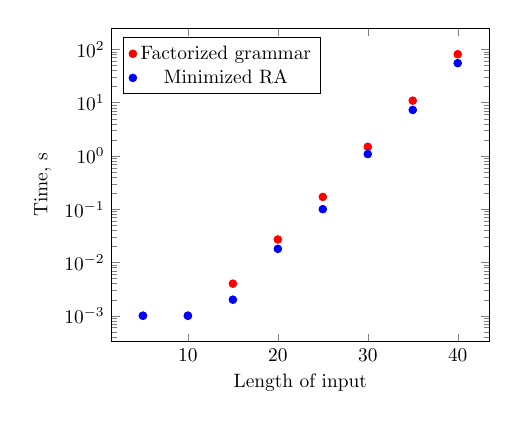
\begin{tikzpicture}[scale=0.7]
        \begin{axis}[
        legend pos = north west,
        xlabel = {Length of input},
        ylabel = {Time, s},
        ymode=log
        ]
        \addplot [only marks, red] coordinates {
            (5,0.001) (10,0.001) (15,0.004) (20,0.027) (25,0.17) (30,1.486) (35,10.9) (40,81.2)
        };
        \addplot [only marks, blue] coordinates {
            (5,0.001) (10,0.001) (15,0.002) (20,0.018) (25,0.1) (30,1.084) (35,7.3) (40,55.2)
        };
        \legend{ 
            Factorized grammar, 
            Minimized RA
        };
        \end{axis}
        \end{tikzpicture}
        \label{fig:Time}
    }
    \caption{Experiments results(1).}
    \label{expPlots1}
\end{figure}